%
% this file is encoded in utf-8
% v1

\documentclass[12pt,a4paper]{ntub_report}

\usepackage{fontspec}   % 加這個就可以設定字體 
\usepackage{xeCJK}      % 讓中英文字體分開設置

% fontset=none因本地端字型有Bug,且也不需用到ctex字體,主要用在修改成章跟節(目錄以及標題)
\usepackage[fontset=none, UTF8, heading=true]{ctex}

% \usepackage{showframe} % 查看排版debug用 makes the page borders visible

%設定主要字型,也就是英文字型
\setmainfont{TimesNewRoman.ttf}% 上網抓ttf

%設定中文字型
%參考 https://www.overleaf.com/learn/latex/Questions/What_OTF/TTF_fonts_are_supported_via_fontspec%3F#Chinese
\setCJKmainfont{mingliu.ttc}% 設定內文為新細明體(沒有內建的),使用W11新細明體字型
\setCJKfamilyfont{kai}{kaiu.ttf}[AutoFakeBold=3]% 設定標楷體直接使用TW-Kai也是一樣,使用W11標楷體字型

% 設置段落自動換行
\XeTeXlinebreaklocale "zh"
\XeTeXlinebreakskip = 0pt plus 1pt

% 目錄跟自動編號的深度(章、節)
\setcounter{tocdepth}{2}
\setcounter{secnumdepth}{2}

% https://www.overleaf.com/learn/latex/Hyperlinks
\usepackage{hyperref}
\hypersetup{
    colorlinks=true,
    linkcolor=black, 
    filecolor=black,      
    urlcolor=black,
    citecolor=black,
    pdfpagemode=FullScreen,
    linktoc=all, % 強制所有標題鏈接有效
    pdftitle={thesis}, %之後改成論文題目
}

% % debug
% \hypersetup{
%     colorlinks=true,
%     linkcolor=blue,
%     filecolor=blue,
%     urlcolor=blue,
%     citecolor=blue,
%     pdfpagemode=FullScreen,
%     linktoc=all,
%     pdftitle={thesis}
% }

%
% this file is encoded in utf-8
% v1

% 除非校方修改了論文格式 (margins, header, footer, 浮水印)
% 或者需要增加所用的 LaTeX 套件,
% 或者要改預設中文字型、編碼
% 否則毋須修改本檔內容
% 論文撰寫,請修改以 my_  開頭檔名的各檔案

\usepackage{titletoc}
\usepackage{geometry}  % for easy margin settings
\usepackage{subfigure}  % for subfigure
\usepackage{multirow}
\usepackage{graphicx}  % for graphic   using eps

%\usepackage{epstopdf} % 當使用pdflatex時打開,如使用latex則不需開啟,此功能為將xxx.eps 自動判讀為XXX.pdf

% \usepackage{subfig} 
\usepackage{algorithmic}  %演算法使用
\usepackage{algorithm}

%
% margins setting
% \geometry{verbose,a4paper,tmargin=3cm,bmargin=3cm,lmargin=3.5cm,rmargin=3cm}
%
\usepackage{amsmath} % 各式 AMS 數學功能
\usepackage{amssymb} % 各式 AMS 數學符號
\usepackage{mathrsfs} %草寫體數學符號,在數學模式裡用 \mathscr{E} 得草寫 E
\usepackage{listings} % 程式列表套件
%
% listing setting
\lstset{breaklines=true,% 過長的程式行可斷行
extendedchars=false,% 中文處理不需要 extendedchars
texcl=true,% 中文註解需要有 TeX 處理過的 comment line, 所以設成 true
comment=[l]\%\%,% 以雙「百分號」做為程式中文註解的起頭標記,配合 MATLAB
basicstyle=\,% 小號字體, 約 10 pt 大小
commentstyle=\upshape,% 預設是斜體字,會影響註解裏的英文,改用正體
%language=Octave % 會將一些 octave 指令以粗體顯示
}

\usepackage{url} % 在文稿中引用網址,可以用 \url{http://www.ntub.edu.tw} 方式

% 插圖套件 graphicx
% 使用者工作流程是用 pdftex 還是 latex + dvipdfmx?
% 視情況而有不同的參數
% 這裡作自動判斷
% 參考自
% http://www.tex.ac.uk/cgi-bin/texfaq2html?label=ifpdf
%\newcommand\mydvipdfmxflow{dvipdfmx}
%\newcommand\mypdftexflow{pdftex}
%
%\ifx\pdfoutput\undefined
%  % not running pdftex
%  \usepackage[dvipdfm]{graphicx}
%  \newcommand\myworkflow{dvipdfmx}  % set the flag for hyperref
%\else
%  \ifx\pdfoutput\relax
%    % not running pdftex
%    \usepackage[dvipdfm]{graphicx}
%    \newcommand\myworkflow{dvipdfmx}  % set the flag
%  \else
%    % running pdftex, with...
%    \ifnum\pdfoutput>0
%      % ... PDF output
%      \usepackage[pdftex]{graphicx}
%      \newcommand\myworkflow{pdftex}  % set the flag
%    \else
%      %...DVI output
%      \usepackage[dvipdfm]{graphicx}
%      \newcommand\myworkflow{dvipdfmx}  % set the flag
%    \fi
%  \fi
%\fi

\usepackage{fancyhdr}  % 借用增強功能型 header 套件來擺放浮水印 
% (佔用了 central header)
% 不需要浮水印的使用者仍可利用此套件,產生所需的 header, footer
%
% 啟動 fancy header/footer 套件
\pagestyle{fancy}
\fancyhead{}  % reset left, central, right header to empty
\fancyfoot[C]{\thepage} %中間 footer 擺放頁碼
\renewcommand{\headrulewidth}{0pt} % header 的直線; 0pt 則無線

% 如果不需要任何浮水印,則請把下列介於 >>> 與 <<< 之間
% 的文字行關掉 (行首加上百分號)
%% 浮水印 >>> 
% %
% this file is encoded in utf-8
% v1.7
% 如果浮水印不是全篇需要,請把下列介於 >>> 與 <<<
% 的「全篇浮水印專用碼」關掉 (行首加百分號)
% 參考自 Keith Reckdahl 寫的 "Using Imported Graphics in LATEX2e" (epslatex.pdf) p.39
% 如果只有特定頁需要浮水印
% 則依該頁屬性使用下列之一的命令 
% 普通頁命令 \thispagestyle{WaterMarkPage}
% plain 頁命令 \thispagestyle{PlainWaterMarkPage}
% empty 頁命令 \thispagestyle{EmptyWaterMarkPage}


% 將重複使用的浮水印章
% 圖檔是 my_watermark.xxx
% 副檔名可以不加,可以是 latex 系統能處裡的任何格式:pdf, gif, png, jpg, eps, ...
% 某些圖檔格式在某些工作流程可能需要作前置處裡。
% 例如,pdflatex 無法直接處理 eps 檔
%  latex + dvipdfmx 無法直接處理 pdf, gif, png, jpg, 需要用 ebb 小工具程式
%  對圖檔產生 .bb 對應檔。
% old code
%\newsavebox{\mywatermark}
%\sbox{\mywatermark}{\includegraphics[keepaspectratio,%
%height=0.8\textheight,%
%width=0.8\textwidth]{my_watermark}}
% new code
\newsavebox{\mywatermark}
%7/23
\sbox{\mywatermark}{
\includegraphics[keepaspectratio,
width=2.5cm]{watermark/ntub_watermark.eps}}


% 將 central header 擺放浮水印的巨集指令
\newcommand{\PlaceWaterMark}{\fancyhead[C]{\setlength{\unitlength}{1in}%
\begin{picture}(0,0)%
%\put(-2.2,-6){\usebox{\mywatermark}}% old code
\put(-0.5,-5.3){\usebox{\mywatermark}}% new code
\end{picture}}%
}

\fancyhead{}  % reset left, central, right header to empty
%% 如果不需整篇論文都要浮水印
%% 則下面  >>> 與 <<< 之間的程式碼請關閉
%% >>> 全篇浮水印

\PlaceWaterMark  % 每一頁都有浮水印 (除了 plain、empty 頁以外)

% 重新定義 plain 頁面
% 每張 plain 頁面 (每一章的第一頁) 也加浮水印

\fancypagestyle{plain}{%
\fancyhead{}%
\PlaceWaterMark%
\fancyfoot{}%
\fancyfoot[C]{\thepage}
\renewcommand{\headrulewidth}{0pt}%
\renewcommand{\footrulewidth}{0pt}%
}
%% <<< 全篇浮水印

%% 如果只有一、兩頁需要有浮水印
%% 可以在該頁 (有頁碼) 使用 \thispagestyle{WaterMarkPage}
%% 此命令不影響原有的 header、footer
\fancypagestyle{WaterMarkPage}{%
\PlaceWaterMark%
}

%% 如果只有一、兩頁 plain 頁需要有浮水印 (如 摘要、自傳等)
%% 可以在該頁 (有頁碼) 使用 \thispagestyle{PlainWaterMarkPage}
%% 只有頁碼與浮水印,沒有其他的 header、footer
%% 等同於 plain page style + water mark
\fancypagestyle{PlainWaterMarkPage}{%
\fancyhead{}%
\PlaceWaterMark%
\fancyfoot{}%
\fancyfoot[C]{\thepage}
\renewcommand{\headrulewidth}{0pt}%
\renewcommand{\footrulewidth}{0pt}%
}

%% 如果只有一、兩頁 empty 頁需要有浮水印 (如封面、書名頁)
%% 可以在該頁 (無頁碼) 使用 \thispagestyle{EmptyWaterMarkPage}
%% 等同於 empty page style + water mark
\fancypagestyle{EmptyWaterMarkPage}{%
\fancyhead{}%
\PlaceWaterMark%
\fancyfoot{}%
\renewcommand{\headrulewidth}{0pt}%
\renewcommand{\footrulewidth}{0pt}%
}

%% <<< 浮水印

% global page layout
\newcommand{\mybaselinestretch}{2}  %行距 1.5 倍 --> 設定 2 看起來比較像1.5倍
\renewcommand{\baselinestretch}{\mybaselinestretch}  % 論文行距預設值
% \parskip=2ex  % 段落之間的間隔為兩個 x 的高度

%%%%%%%%%%%%%%%%%%%%%%%%%%%%%
%  end of preamble
%%%%%%%%%%%%%%%%%%%%%%%%%%%%%


% 目錄無法超連結棄用
% % 自定義 章節(包含目錄)
% % 參考
% % https://www.ptt.cc/bbs/LaTeX/M.1247243154.A.5E9.html
% % https://lzsh00262.blogspot.com/2013/02/xelatex.html
% \usepackage{titlesec,titletoc,CJKnumb}
% \renewcommand{\thechapter}{\arabic{chapter}}
% \renewcommand{\thesection}{\arabic{section}}

% % font size (relative to 12 pt):
% % Large (18pt) < \LARGE (20pt)
% % 20pt 標楷體(禁用粗體效果,使用 \mdseries 恢復正常字重)
% \titleformat{\chapter}{\centering\fontsize{20pt}{20pt}\mdseries\CJKfamily{kai}}{}{0em} {}
% \titlespacing{\chapter}{0cm}{-1cm}{0em}

% % 18pt 標楷體(禁用粗體效果,使用 \mdseries 恢復正常字重)
% \titleformat{\section}{\centering\fontsize{18pt}{18pt}\mdseries\CJKfamily{kai}}{}{0em} {}
% \titlespacing{\section}{0cm}{0cm}{1em}

% % 目錄新細明體
% \titlecontents{chapter}[0em]
%               {}{\normalfont\normalsize\makebox[3.4em][l]
%               {第\CJKnumber{\thecontentslabel}章\quad}}{}
%               {\titlerule*[0.7pc]{.}\contentspage}
% \titlecontents{section}[1em]
%               {}{\normalfont\normalsize\makebox[3.4em][l]
%               {第\CJKnumber{\thecontentslabel}節\quad}}{}
%               {\titlerule*[0.7pc]{.}\contentspage}

% 插入論文口試委員審定書、無違反學術倫理聲明書用
% \usepackage{pdfpages}
  %基本的環境設定  無需改變

%參考文獻APA格式,記得在bib加上 keywords  = {chinese} or {english}
\usepackage[style=apa]{biblatex} % 'backend=biber' is the default
\addbibresource{my_bib.bib}

\begin{document}



	% 下列中文名詞的定義,如果以註解方式關閉取消,
% 則會以系統原先的預設值 (英文) 替代
% 名詞 \prechaptername 預設值為 Chapter
% 名詞 \postchaptername 預設值為空字串
% 名詞 \tablename 預設值為 Table
% 名詞 \figurename 預設值為 Figure


%\renewcommand\prechaptername{第} % 出現在每一章的開頭的「第 x 章」
%\renewcommand\postchaptername{章}

\ctexset{
    chapter = {
        name = {第,章},
        number = \chinese{chapter},
        format = \centering\CJKfamily{kai}\fontsize{20}{20}\selectfont\textbf,  % 設定字體為標楷體並且大小為20pt
        beforeskip = -24pt,  % 章標題前的間距
        afterskip = 0pt,  % 章標題後的間距
    },
    section = {
        name = {第,節},
        number = \chinese{section},
        format = \centering\CJKfamily{kai}\fontsize{18}{18}\selectfont\textbf,  % 調整字體與大小
        beforeskip = 0pt,  % 調整節標題前的空間
        afterskip = 0pt,  % 節標題與正文之間無空行
    },
    subsection = {
        format = \raggedright\CJKfamily{kai}\fontsize{16}{16}\selectfont\textbf,
        beforeskip = 0pt,
        afterskip = 0pt,
    },
    subsubsection = {
        format = \raggedright\CJKfamily{kai}\fontsize{14}{14}\selectfont\textbf,
        beforeskip = 0pt,
        afterskip = 0pt,
    },
}

\renewcommand{\tablename}{表} % 在文章中 table caption 會以「表 x」表示
\renewcommand{\figurename}{圖} % 在文章中 figure caption 會以「圖 x」表示

% 下列中文名詞的定義,用於論文固定的各部分之命名 (出現於目錄與該頁標題)
\newcommand{\nameInnerCover}{教授推薦書}
\newcommand{\nameCommitteeForm}{論文口試委員審定書}
\newcommand{\nameCopyrightForm}{授權書}
\newcommand{\nameCabstract}{\hspace{1em}摘\hspace{1em}要}
\newcommand{\nameEabstract}{\hspace{1em}ABSTRACT}
\newcommand{\nameAckn}{\hspace{1em}誌\hspace{1em}謝}
\newcommand{\nameToc}{\hspace{1em}目\hspace{1em}錄}
\newcommand{\nameTof}{\hspace{1em}圖目錄}
\newcommand{\nameLot}{\hspace{1em}表目錄}
\newcommand{\nameToa}{演算法目錄}
\newcommand{\nameSlist}{符號說明}
\newcommand{\nameRef}{參考文獻}
\newcommand{\nameVita}{自傳}
 %在此檔案處定義文章中的中文名詞

	%---------------------------------------------------------------------------------------------------------
	%%% 以下是載入前頁、本文、後頁

	%---------------------------------------------------------------------------------------------------------
	% front matter 前頁
	% 包括封面、書名頁、中文摘要、英文摘要、誌謝、目錄、表目錄、圖目錄、符號說明
	% 在撰寫各章草稿時,可以把此部份「關掉」,以節省無謂的編譯時間。
	% 實際內容由
	%    my_names.tex, my_cabstract.tex, my_eabstract.tex, my_ackn.tex, my_symbols.tex
	% 決定
	% ntust_frontpages.tex 此檔只提供整體架構的定義,不需更動
	% 在撰寫各章草稿時,可以把此部份「關掉」,以節省無謂的編譯時間。
	
	%
% this file is encoded in utf-8
% v1

\pagestyle{plain}  % 前幾頁不顯示 fancyhdr

% 無須修改本檔內容,除非校方修改了
% 封面、書名頁、中文摘要、英文摘要、誌謝、目錄、表目錄、圖目錄、符號說明
% 等頁之格式

% make the line spacing in effect
% \renewcommand{\baselinestretch}{\mybaselinestretch}
% \large % it needs a font size changing command to be effective

% default variables definitions
% 注意!!此處只是預設值,不需更改此處
% 請更改 my_names.tex 內容
\newcommand\cTitle{論文題目}
\newcommand\eTitle{MY THESIS TITLE}
\newcommand\myCname{OOO}
\newcommand\advisorCnameA{OOO\ 博士}
\newcommand\univCname{國立臺灣大學}
\newcommand\deptCname{資訊工程研究所}
\newcommand\degreeCname{碩士}
\newcommand\cYear{一一四}
\newcommand\cMonth{六}

 % user's names; to replace those default variable definitions
%
% this file is encoded in utf-8
% v1
% 填入你的論文題目、姓名等資料
% 如果題目內有必須以數學模式表示的符號,請用 \mbox{} 包住數學模式

% 論文題目 (中文)
\renewcommand\cTitle{%我的碩士論文題目 
論文題目
}

% 論文題目 (英文)
\renewcommand\eTitle{%My Thesis Title  
My Thesis Title
% My Thesis Title  \mbox{$\cal{H}_\infty$} and \mbox{Al$_x$Ga$_{1-x}$As}
}

% 我的姓名 (中文)
\renewcommand\myCname{你(妳)的名字}

% 指導教授A的姓名 (中文)
\renewcommand\advisorCnameA{指導教授的姓名\ 博士}

% 校名 (中文)
\renewcommand\univCname{國立臺北商業大學管理學院}

% 系所名 (中文)
\renewcommand\deptCname{資訊管理系人工智慧與商業應用碩士班}

% 學位名 (中文)
\renewcommand\degreeCname{碩士學位}

% 口試年份 (中文、民國)
\renewcommand\cYear{一一四}

% 口試月份 (中文)
\renewcommand\cMonth{六} 

%畢業級別;用於書背列印;若無此需要可忽略
\newcommand\GraduationClass{114}

%%%%%%%%%%%%%%%%%%%%%%
%%%%%%%%%%%%%%%%%%%%%%%%%%%%%%%
%       ntust cover 封面
%%%%%%%%%%%%%%%%%%%%%%%%%%%%%%%
%
% this file is encoded in utf-8
% v1

\newgeometry{top=2cm, bottom=2cm, left=2cm, right=2cm}

%%%%%%%%%%%%%%%%%%%%%%%%%%%%%%%
%       ntust cover 封面
%%%%%%%%%%%%%%%%%%%%%%%%%%%%%%%
%
\begin{titlepage}
% no page number
% next page will be page 1

% aligned to the center of the page horizontally
\begin{center}
% font size (relative to 12 pt):
% \large (14pt) < \Large (18pt) < \LARGE (20pt) < \huge (24pt)< \Huge (24 pt)
%
% 校名與系所名
% \vspace*{0cm}
{\CJKfamily{kai}\fontsize{26pt}{26pt}\selectfont\textbf{\univCname}}\\ % 校名,26pt
\vspace{0.25cm}
{\CJKfamily{kai}\fontsize{24pt}{36pt}\selectfont\textbf{\deptCname}}\\ % 系所名,24pt
\vspace{0.25cm}
{\CJKfamily{kai}\fontsize{24pt}{36pt}\selectfont\textbf{\degreeCname 論文}}\\ % 論文種類,24pt
\vspace{0.25cm}
%
\vspace{18pt}
\vspace{18pt}
\vspace{18pt}
\vspace{18pt}
\vspace{18pt}
%
{\CJKfamily{kai}\fontsize{24pt}{36pt}\selectfont\textbf{\cTitle}}\\ % 論文種類,24pt
\fontsize{22pt}{22pt}\selectfont{\eTitle}\\ % 英文題目,20pt 或 22pt,Times New Roman
%
\vspace{12pt}
\vspace{12pt}
\vspace{12pt}
\vspace{12pt}
\vspace{12pt}
\vspace{12pt}
\vspace{12pt}
\vspace{12pt}
\vspace{12pt}
\vspace{12pt}
%
% 研究生與指導教授信息
{\CJKfamily{kai}\fontsize{18pt}{18pt}\selectfont\textbf{{研究生:\Large{\myCname}}}}\\ % 研究生,18pt
\vspace{18pt}
\vspace{18pt}
\vspace{18pt}
\vspace{18pt}
{\CJKfamily{kai}\fontsize{18pt}{18pt}\selectfont\textbf{指導教授:\Large{\advisorCnameA}}}\\ % 指導教授A,18pt
\vspace{18pt}
\vspace{18pt}
\vspace{18pt}
% 顯示日期 18pt
{\CJKfamily{kai}\fontsize{18pt}{18pt}\selectfont\textbf{中華民國\cYear 年\cMonth 月}}\\
%
\end{center}
% 恢復原設置
% \renewcommand{\baselinestretch}{\mybaselinestretch}   %恢復原設定
% % restore the font size to normal
% \normalsize
\end{titlepage}
%%%%%%%%%%%%%%

%%%%%%%%%%%%%%

\newgeometry{top=3cm, bottom=3cm, left=3.5cm, right=3cm}

%% 從摘要到本文之前的部份以小寫羅馬數字印頁碼
% 但是從「書名頁」(但不印頁碼) 就開始計算
%\setcounter{page}{1}
\pagenumbering{Roman}
%\pagenumbering{arabic}

% 判斷是否要浮水印?
\ifx\mywatermark\undefined 
  \thispagestyle{empty}  % 無頁碼、無 header (無浮水印)
\else
  \thispagestyle{EmptyWaterMarkPage} % 無頁碼、有浮水印
\fi

%%%%%%%%%%%%%%%%%%%%%%%%%%%%%%%%%%%%%%%%%%%%%%%%%%%%%%%%%%%%%%%


%%%%%%%%%%%%%%%%%%%%%%%%%%%%%%%%%%%%%%%%%%%%%%%%%%%%%%%%%%%%%%%%%%%%%
%%%%%%%%%%%%%%%%%%%%%%%%%%%%%%%
%       論文口試委員審定書、無違反學術倫理聲明書(不顯示頁碼、目錄)
%%%%%%%%%%%%%%%%%%%%%%%%%%%%%%%
%
% insert the printed standard form when the thesis is ready to bind
% 在口試完成後,再將已簽名的審定書、聲明書放入以便裝訂
% create an entry in table of contents for 審定書、聲明書

% % 插入審定書 PDF(假設檔名為 approval.pdf)
% \cleardoublepage
% \includepdf[pages=-, pagecommand={\thispagestyle{empty}}]{frontpages/forms/口試審定書-簽名版.pdf}

% % 插入學術倫理聲明書 PDF(假設檔名為 ethics.pdf)
% \cleardoublepage
% \includepdf[pages=-, pagecommand={\thispagestyle{empty}}]{frontpages/forms/無違反學術倫理聲明書-簽名版.pdf}

% ↓ 在插入完兩個 PDF 後,重設頁碼計數
% \cleardoublepage
% \setcounter{page}{1}
% \pagenumbering{Roman}

%%%%%%%%%%%%%%%%%%%%%%%%%%%%%%%
%       中文摘要 
%%%%%%%%%%%%%%%%%%%%%%%%%%%%%%%
%
% aligned to the center of the page
\chapter*{\mdseries\nameCabstract}
% create an entry in table of contents for 中文摘要
% \addcontentsline{toc}{chapter}{ \nameCabstract}
\addcontentsline{toc}{chapter}{\nameCabstract}
\thispagestyle{plain}  % 無 header,但在浮水印模式下會有浮水印
% \vspace*{0.5cm}
% Resume the line spacing to the desired setting
\renewcommand{\baselinestretch}{\mybaselinestretch}   %恢復原設定
%it needs a font size changing command to be effective
% restore the font size to normal
\normalsize
%%%%%%%%%%%%%

分散式詢問及監督系統主要被用於分散式資料如檔案或是紀錄的維護上。網路內的使用者可以自系統中查詢所需資料如總和或平均值,若同時將所有原始資料做傳遞及運算,將耗費相當大的網路頻寬及運算資源。於是,內網路聚集技術被提出來降低分散式詢問及監督系統的負擔。然而,這個技術卻容易遭受安全威脅。過去的研究大多假設資料來源為可信任,並針對聚集架構進行安全性的研究。然而,我們認為聚集查詢結果應該在面對惡意攻擊者將錯誤資料置入資料串流進行聚集前,就應該具備強健的容錯能力。傳統上,一個強健的估計值被定義為即使資料來源有誤時,亦能維持一定程度正確性的聚集結果。許多常見的強健估計值是建立在有序統計學上,因此,我們將重心放在內網路計算上之有序統計的可驗證技術。此技術的挑戰為在網路遭受惡意團體介入聚集程序時,仍能確保聚集結果或近似結果的準確性。
	
\vspace{1em}
\vspace{1em}
\vspace{1em}
\noindent 關鍵字:OOO

%%%%%%%%%%%%%%%%%%%%%%%%%%%%%%%
%       英文摘要 
%%%%%%%%%%%%%%%%%%%%%%%%%%%%%%%
%
% aligned to the center of the page
\chapter*{\mdseries\nameEabstract}
% create an entry in table of contents for 中文摘要
% \addcontentsline{toc}{chapter}{ \nameEabstract}
\addcontentsline{toc}{chapter}{\nameEabstract}
\thispagestyle{plain}  % 無 header,但在浮水印模式下會有浮水印
% \vspace*{0.5cm}
% Resume the line spacing to the desired setting
\renewcommand{\baselinestretch}{1.5}   %恢復原設定
%it needs a font size changing command to be effective
% restore the font size to normal
\normalsize
%%%%%%%%%%%%%
Distributed querying and monitoring systems have been widely studied in recent years. These systems aim to maintain data sources, such as data set or log files, and allow users to query over those data sources. When the data sources are highly related and users only care some statistic results, like the sum or the average, it is consumed to transmit all data sources via the network. To minimize the network consumption, in-network aggregation technique is proposed. However, this technique is subject to some known attacks, such as the injection attack and the pollution attack. Prior works only considered the settings that data sources are trusted while the network is not. We study the way to relax the limitation and guarantee the aggregate queries robust to malicious or faulty data sources (also called polluted data sources). 

\vspace{1em}
\vspace{1em}
\vspace{1em}
\noindent Keywords:OOO

%%%%%%%%%%%%%%%%%%%%%%%%%%%%%%%
%       誌謝 
%%%%%%%%%%%%%%%%%%%%%%%%%%%%%%%
%
% Acknowledgment
% aligned to the center of the page
\chapter*{\mdseries\nameAckn}
% create an entry in table of contents for 中文摘要
% \addcontentsline{toc}{chapter}{ \nameAckn}
\addcontentsline{toc}{chapter}{\nameAckn}
\thispagestyle{plain}  % 無 header,但在浮水印模式下會有浮水印
% \vspace*{0.5cm}
% Resume the line spacing to the desired setting
\renewcommand{\baselinestretch}{\mybaselinestretch}   %恢復原設定
%it needs a font size changing command to be effective
% restore the font size to normal
\normalsize
%%%%%%%%%%%%%

	首先誠摯的感謝指導教授陳明明博士,老師悉心的教導使我得以一窺WSN的深奧,不時的討論並指點我正確的方向,使我在這些年中獲益匪淺。老師對學問的嚴謹更是我輩學習的典範。
    本論文的完成另外亦得感謝老師們大力協助。因為有你們的體諒及幫忙,使得本論文能夠更完整而嚴謹。
 兩年裡的日子,實驗室裡共同的生活點滴,學術上的討論、言不及義的閒扯、讓人又愛又怕的宵夜、趕作業的革命情感、因為睡太晚而遮遮掩掩閃進實驗室........,感謝眾位學長姐、同學、學弟妹的共同砥礪,你/妳們的陪伴讓兩年的研究生活變得絢麗多彩。
	最後絕對不能忘記最了解、最支持我的家人─我的父親、母親及姊姊,在我喪失動力之時,隨時都能給予我心靈上無窮盡的關心與鼓勵,讓我有勇氣堅持到最後,完成研究的旅途。還有很多曾經幫助過我的朋友,因為有大家的幫助,我才能有今天的成果。想要感謝的人真的太多太多,就只有感謝上天了!






% Resume the line spacing to the desired setting
\renewcommand\addvspace[1]{}

%%%%%%%%%%%%%%%%%%%%%%%%%%%%%%%
%       目錄 
%%%%%%%%%%%%%%%%%%%%%%%%%%%%%%%
%
% Table of contents
\newpage
\renewcommand{\contentsname}{\mdseries\nameToc}
\phantomsection % for hyperref to register this
% \addcontentsline{toc}{chapter}{ \nameToc}
\addcontentsline{toc}{chapter}{\nameToc}
\tableofcontents



%%%%%%%%%%%%%%%%%%%%%%%%%%%%%%%
%       圖目錄 
%%%%%%%%%%%%%%%%%%%%%%%%%%%%%%%
%
% List of Figures
\newcommand{\loflabel}{圖}
\newpage
\renewcommand{\numberline}[1]{\loflabel~#1\hspace*{1em}}
\renewcommand{\listfigurename}{\mdseries\nameTof}
\phantomsection % for hyperref to register this
% \addcontentsline{toc}{chapter}{ \nameTof}
\addcontentsline{toc}{chapter}{\nameTof}
\listoffigures


%%%%%%%%%%%%%%%%%%%%%%%%%%%%%%%
%       表目錄 
%%%%%%%%%%%%%%%%%%%%%%%%%%%%%%%
%
% List of Tables
\newcommand{\lotlabel}{表}
\newpage
\renewcommand{\numberline}[1]{\lotlabel~#1\hspace*{1em}}
\renewcommand{\listtablename}{\mdseries\nameLot}
\phantomsection % for hyperref to register this
% \addcontentsline{toc}{chapter}{ \nameLot}
\addcontentsline{toc}{chapter}{\nameLot}
\listoftables

%%%%%%%%%%%%%%%%%%%%%%%%%%%%%%%
%       演算法目錄 
%%%%%%%%%%%%%%%%%%%%%%%%%%%%%%%
%
% List of Figures
%\newpage
%\renewcommand{\listalgorithmname}{\protect\makebox[5cm][s]{\nameToa}}
%\makebox{} is fragile; need protect
%\addcontentsline{toc}{chapter}{\nameToa}
%\listofalgorithms


%%%%%%%%%%%%%%%%%%%%%%%%%%%%%%%
%       符號說明 
%%%%%%%%%%%%%%%%%%%%%%%%%%%%%%%
%
% Symbol list
% define new environment, based on standard description environment
% adapted from p.60~64, <<The LaTeX Companion>>, 1994, ISBN 0-201-54199-8
%\newcommand{\SymEntryLabel}[1]%
% {\makebox[3cm][l]{#1}}
%
%\newenvironment{SymEntry}
%   {\begin{list}{}%
%       {\renewcommand{\makelabel}{\SymEntryLabel}%
%        \setlength{\labelwidth}{3cm}%
%        \setlength{\leftmargin}{\labelwidth}%
%        }%
%   }%
%   {\end{list}}
%%
%\newpage
%\chapter*{\protect\makebox[5cm][s]{\nameSlist}} %\makebox{} is fragile; need protect
%\addcontentsline{toc}{chapter}{\nameSlist}
%%
% this file is encoded in utf-8
% v1
%  各符號以 \item[] 包住,然後接著寫說明
% 如果符號是數學符號,應以數學模式表示,以取得正確的字體
% 如果符號本身帶有方括號,則此符號可以用大括號 {} 包住保護
\begin{SymEntry}

\item[OLED]
Organic Light Emitting Diode

\item[$E$]
energy

\item[$e$]
the absolute value of the electron charge, $1.60\times10^{-19}\,\text{C}$
 
\item[$\mathscr{E}$]
electric field strength (V/cm)

\item[{$A[i,j]$}]
the  element of the matrix $A$ at $i$-th row, $j$-th column\\
矩陣 $A$ 的第 $i$ 列,第 $j$ 行的元素

\end{SymEntry}

% Resume the line spacing to the desired setting
\renewcommand{\baselinestretch}{\mybaselinestretch}   %恢復原設定
%it needs a font size changing command to be effective
% restore the font size to normal
\normalsize

%% 論文本體頁碼回復為阿拉伯數字計頁,並從頭起算
\newpage
\setcounter{page}{1}
\pagenumbering{arabic}

\pagestyle{fancy}
\fancyhf{}
\fancyfoot[C]{\ifnum\value{page}>0 第 \thepage 頁,共 \pageref{LastPage} 頁\fi}

% 確保 plain 頁碼格式(如章節首頁)也適用 fancyhdr
\fancypagestyle{plain}{%
    \fancyhf{}
    \fancyfoot[C]{第 \thepage 頁,共 \pageref{LastPage} 頁}
}
%%%%%%%%%%%%%%%%%%%%%%%%%%%%%%%% 




	%---------------------------------------------------------------------------------------------------------
	% main body 論文主體。建議以「章」為檔案分割的依據。
	% 以下為建議的命名分類
	%   introduction.tex   related_work.tex  protocol.tex  evaluation.tex  conclusion.tex
	% 做為這幾個「章」的檔案名稱,並將檔案存放於資料夾 sections/ 下
	% 實際命名方式可以隨你意
	% 在撰寫各章草稿時,可以把其他章節關掉 (行首加百分號)
	%%
% this file is encoded in utf-8
% v1.7
\chapter{\mbox{\LaTeX\ 示範}}
\label{ch:example}
這一章目的是一些基本功能的用法。最好是與原始檔案 example\_body.tex 一起對照著看。章節標題後之第一段之段首不需要內縮。

如何顯示圖檔?
圖~\ref{fig:logo} 是元智大學的校徽,以保持長寬比例,寬 2~cm,中間對齊顯示。插圖的標題須在圖的下方。如果是從別的文獻引用,出處則註記於圖標題下方。
\begin{figure}[htbp]
\centering 
\includegraphics[%
  width=2cm,keepaspectratio]{example/example_fig}
\caption{\label{fig:logo}校徽 The logo.}
(This logo comes from the school web page.)
\end{figure}

如何顯示表格?表~\ref{tb:income_2003} 是示範簡易的 $3\times3$ 的表格,除了第一欄是中間對齊以外,第二、三欄是向右對齊。表格的標題須在表格上方。或者,使用只有橫線的表格,如表~\ref{tb:income_2003_v2}。資料的出處則註記於表格下方。
%
\begin{table}[htbp]
\caption{\label{tb:income_2003}Gross income of the first two quarters of
year 2003.}
\centering \begin{tabular}{|c|r|r|}
\hline 
&
Restaurant&
Store\tabularnewline
\hline
\hline 
Q1&
\$123,000&
\$75,000\tabularnewline
\hline 
Q2&
\$45,000&
\$131,000\tabularnewline
\hline
\end{tabular}\\
(This table is made up for demonstration purpose.)
\end{table}%
%
\begin{table}[htbp]
\caption{\label{tb:income_2003_v2}Gross income of the first two quarters of
year 2003. Version 2.}
\centering \begin{tabular}{crr}
\hline 
&
Restaurant&
Store\tabularnewline
\hline
Q1&
\$123,000&
\$75,000\tabularnewline
 Q2&
\$45,000&
\$131,000\tabularnewline
\hline
\end{tabular}\\
(This table is made up for demonstration purpose.)
\end{table}


現在來示範參考文獻的引用。根據文獻\cite{ieee_dmr_2_50_2002_chou} 的說法,此實驗必須湊齊五大元素\cite{jap_093_1108_2003_kondakov, ieee_ed_50_1830_2003_oriols, Chem.Mater._8_1365_1996_Papadimitrakopoulos, jap_079_2745_1996_scott, jap_087_8049_2000_adachi, jap_089_1704_2001_brutting, jap_089_4673_2001_popovic, synth.met._132_9_2002_nomura, cjk_book, thinfilm_macleod_2001},並用天火燒之始能畢其功。


\chapter{數學式子}
我們在第 \pageref{ch:example} 頁示範了如何處理插圖以及表格。在這一章,我們來看數學公式的處理。在本文行內要書寫數學符號、式子,可以用錢符號前後包夾住表示式。如 \$ax+b=0\$ 會顯示 $ax+b=0$;如果要單獨展示數學公式,則用 \verb+\[+ 以及 \verb+\]+ 包夾住表示式。如下
\[
\sum_{k=1}^{\infty}\frac{1}{n^2}
\]

如果公式要編號碼,則要用\verb+\begin{equation}+ 以及 \verb+\end{equation}+,並在式子中加上 \verb+\label{}+ 的標籤。如
\begin{equation}
  \frac{df}{dx} \equiv \lim_{\Delta x \rightarrow 0} \frac{f(x+\Delta x) - f(x)}{\Delta x}   \label{eq:diff_def}
\end{equation}
我們可以在公式 (\ref{eq:diff_def}) 看到微分的定義。

可以參考李果正先生寫的《大家來學 {\LaTeX}》,學習更多的技巧。\\
\textless{}\url{http://edt1023.sayya.org/tex/latex123/index.html}\textgreater{}

\chapter{元智大學論文格式規範}
(本文節自《元智大學研究所學位論文格式規範條例》,文中所提之附件,\\
詳見\textless{}\url{http://www.yzu.edu.tw/admin/1/8_7.htm}\textgreater{})

\section{規格說明}
\begin{description}
\item[封面]  教務處統一格式樣本,如附件一,經教育部核可分組者是否加註組別及封面紙由各所自定。
\item[書名頁] 包括論文中英文名稱,著者及指導教授中英文姓名、校名、所名、學位論文別、提送論文英文說明及地名,提送年月等,如附件二。
\item[口試委員會審定書] 教務處統一格式樣本,如附件四,正本由各所彙整送交教務處,影本裝訂於論文內。
\item[授權書] 無論是否同意開放學術利用,本頁均須裝訂,如附件三,並與提要電子檔案開放使用欄表達一致。 (另有國科會授權書) 
\item[中英文摘要] 內容應說明研究目的,資料來源,研究方法及結果等,約 500--1000 字,並以一頁為限。須有中文摘要及英文摘要,分頁書寫,格式如附件五、六。
\item[論文尺寸及紙張] 以 $210\,\mathrm{mm} \times 297\,\mathrm{mm}$ 規格 A4 紙張繕製。封面封底採用 150 磅以上布紋紙或卡紙,顏色均由各所指定。
\item[版面規格] 紙張頂端留邊 3.5~cm,左側留邊 4~cm,右側留邊 2~cm,底端留邊 2~cm,版面底端 1~cm 處文字版面中心線處繕打頁次。
\item[文字規格] 文章主體以中文為原則,由左至右,橫式打字繕排,文句中引用之外語原文以~(~)~號附註。
\item[頁次] (1) 中文摘要至圖表目錄等,以 i, ii, iii, \ldots\ 等小寫羅馬數字連續編頁。書名頁、審定書雖無須印出頁碼,但仍應編入同此之頁碼。\\
(2) 論文中第一章以至附錄,均以 1, 2, 3, \ldots\ 等阿拉伯數字連續編頁。
\item[裝訂] 自論文本左端裝釘,書背外貼紙邊,打印畢業級別、學位論文別、論文名稱、校、院、所名、著者姓名。 (見附件十八)。
\end{description}

\section{操作細則}

\begin{description}
\item[目錄] 按本規範所訂「論文編印項目次序」各項順序,依次編排論文內各項目名稱、章、節編號、頁次等 (見附件九、九-1,請與指導教授討論擇一採用)。
\item[圖表目錄] 文內表圖,各依應用順序,不分章節連續編號,並表列一頁目次 (見附件十、十一)。
\item[符號說明] 各章節內所使用之數學及特殊符號,均集中表列一頁說明,以便參閱,表內各符號不須編號 (見附件十二)。
\item[論文本文章節編號] 章次使用一、二、⋯⋯ (或第一章、第二章⋯⋯) 等中文數字編號,節段編號則配合使用一、1-1、1-1-1、1.、 (1) 、 (或第一節、第二節、第三節、壹、一、1、(1)) 等層次順序之阿拉伯數字。
\item[論文本文章節名稱及段落層次] (見附件十三、十三-1,請與指導教授討論擇一採用)\\
(1) 章次、章名稱位於打字版面頂端中央處。\\
(2) 節次、段次均自版面左端排起,各空一、二格,繕排名稱。\\
(3) 小段以下等號次及名稱,均以行首空數格間距表明層次。
\item[論文本文行距] 中文間隔一行,每頁最少 32 行,英文間隔 1.5 或 2 行 (1.5 space or double space),每頁最少 28 行,章名下留雙倍行距。
\item[論文本文字距] 中文為密集字距,如本規範使用字距,每行最少 28 字,英文不拘。
\item[論文本文文句內數字運用] 有下列注意事項\\
(1) 描述性、非運算之簡單數字及分數數字,以中文數字表示。例:一百五十人,三萬二仟元,六十分之十七等。\\
(2) 繁長者視情況使用中文或阿拉伯數字,以簡明為宜。例:美金三十三億元 (不用 3,300,000,000 元)。\$15,349 (不用一萬五千三百四十九美元)。
\item[論文本文方程式及公式] 有下列注意事項\\
(1) 方程式及公式應縮格排列,並與正文儘區隔分開。例如:
\[ x = \frac{-b \pm \sqrt{b^2 -4ac}}{2a}. \]\\
(2) 方程式及公式不只一個時應編排序號,該序號應以圓括弧標註於最後一行的最右邊。例如:
\begin{equation}
E = mc^2.
\end{equation}\\
(3) 在正文提到相關之方程式或公式時,須表明該方程式之名稱及序號。\\
(4) 如果方程式較長需轉行時,只能在加、減、乘、除、大於、小於等運算子符號處轉行。上下式儘可能在等號「=」處對齊。例如:
\begin{equation}
\begin{split}
f(x) &= f(0) + f'(0)x + \frac{f''(0)}{2!}x^2 + \frac{f'''(0)}{3!}x^3 +\cdots \\
    &=1+\frac{1}{2}x+\left(-\frac{1}{8}\right)x^{2}+\left(\frac{1}{16}\right)x^{3}+\cdots.
\end{split}
\end{equation}\\
(5) 正文中之分數應使用 ``/'' 以區分分子與分母。例如:1/2。
\item[論文本文註腳] 有下列注意事項\\
(1) 特殊事項論點等,可使用註腳 (Footnote) 說明。\\
(2) 註腳應依順序編號,編號標於相關文右上角%
\footnote{這是 footnote 的例子。}%
以備參閱。各章內編號連續,各章之間不相接續。\\
(3) 註腳號碼及內容繕於同頁底端版面內,與正文之間加劃橫線區隔,頁面不足可延用次頁底端版面。
\item[論文本文文獻參閱] 文中所有參考之文獻,不分中英文及章節,均依參閱順序連續編號,並將參閱編號,加中括號~[~]~號標明於參閱處。文獻資料另編錄於論文本文之後。
\item[論文本文圖表編排] 有下列注意事項\\
(1) 表號及表名列於表上方,圖號及圖名置於圖下方。資料來源及說明,一律置於表圖下方。\\
(2) 圖表內文數字應予打字或以工程字書寫。
\item[參考文獻資料編排] 所有參考文獻資料,均置於論文本文之後,獨立另起一頁,按參閱編號依次編錄,頁次仍以本文接續。
\item[附錄] 凡屬大量數據、推導、註釋有關或其他冗長被參之資料、圖表,均可分別另起一頁,編為各附錄。正文中未引用之參考文獻應列出書目置於附錄之中。
\end{description}

\chapter{兩篇短文}
論文格式規範有些要在一章的第二頁之後,有些要在整頁文字的情況下,有些要在多層次分節的情況下才看得出來。所以,附上兩篇輕鬆的短文,來展示前面各章節還沒有遇到的論文規範。

\section{南橫上的捍衛戰警—閻驊}
\label{speed}
(原文作者為閻驊,見於 \textless{}\url{http://www.1001yeah.com.tw}\textgreater{})

今年舊曆新年前,我進行了兩年來的第五度環島旅行。不過這次遇上了大麻煩!因為汽車在南橫公路接近最高點的地方拋錨。這次拋錨事件讓我非常尷尬!一、我居然在一個接近三十度的險升坡上拋錨!二、汽車拋錨之處,手機居然無法播通!三、就算手機可以播通,其實也沒啥屁用!因為南橫目前是禁止大型車進入,所以拖吊車根本無法開進來救我。那時我直覺地認為應該是汽車沒電、才會拋錨!所以我就開始裝可愛、站在路旁攔車、幫我接電。但是不知道怎麼搞的!在汽車拋錨之後的半小時,南橫似乎道路封閉似的!居然沒有半台汽車經過?半小時之後,當第一台汽車映入眼簾時,就接連著出現了十幾台汽車魚貫而來,每一位駕駛員對我的反應都是一樣的:放慢車速→拉下車窗→看看我的車子→思索三秒鐘→對我搖搖頭→加速離去。整整一小時之後,才出現了第一台願意停下來、幫我忙的車子。車主熱心地把車頭倒過來、幫我接電。結果∼我的笨蛋汽車依然無法發動!我想這下子糟糕了!我可能要宣布棄車逃亡了。

\subsection{發生了什麼事?}
不過這時奇蹟出現了!接連又來了兩台汽車、自動自發地停下來、加入修車的行列中。場面此時開始熱鬧了起來,狹小的南橫公路上停了四台車、十個人一起七嘴八舌地討論了修車方案。

\subsection{修車方法}
正好這些好心人裡頭,有兩位剛從軍中退伍的修車兵。根據他們專業的眼光來看,他們一致認為火星塞應該髒掉了!於是大家用一些很「馬蓋先」的克難方式,有說又笑地把我的引擎拆開,用衛生筷子夾著衛生紙,擦拭其中的一個火星塞%
\footnote{為何會選擇那一個火星塞來修理呢?後來我才知道他們是瞎矇的!因為台南的修車廠老闆告訴我,那一個火星塞是我汽車四個火星塞之中,
唯一沒有故障的那一個!}%
,然後我的汽車就這麼神奇地發動成功了!

 當我的汽車成功發動之後,這些幫我修車的好心人們突然問了我老婆一個問題:「請問你有男友嗎?」。我那誠實的老婆指著我、回答道:「我沒有男友,但是車主是我老公!」。於是這群好心的大男生就長嘆一聲,三台好心車、八位好心人就這麼一瞬間消失無蹤。
 
\subsection{另一項考驗}
不過我的另一個考驗在汽車發動成功之後才登場。這個考驗就是:我的時速不能低於三十公里、不然就會讓我的引擎再度熄火。況且我拋錨的路段距離台南還有兩百公里。而且接下來的路段可是峰迴路轉、路面狹窄!而且單向通車的路段也是不少!這種考驗幾乎就等於是基努李維所飾演的「捍衛戰警」一樣:就是車速一慢,炸彈立即引爆。
 
所以接下來的山路,我都是馬不停蹄地向前狂奔。遇到前方有車,幾乎都是像流氓一樣地猛按喇叭、狠狠超車。如果看到前方是單向通車的路段,我都是硬踩著油門、用超過一百公里的速度火速通過。

兩個多小時之後,我就成功地飆到台南某修車廠、總計開了兩百公里、下降了兩千九百公尺、平均下山時速約九十公里。我的耳膜與心臟都非常地疼痛! (因為車速只要低於六十公里,我的笨蛋汽車就會發出一種非常 Weak 的聲響,提醒我:「主人∼主人,我又要拋錨囉!趕快跳傘逃生吧!」,讓我心力交瘁!) 

捍衛戰警的故事就講到這裡!不過在這個故事裡頭有一個小插曲,讓我感觸良多!我這些日子以來,午夜夢迴時經常會想起。前述文字不是曾經提到,當我汽車拋錨之後的一個小時內,大約有十幾台汽車經過!但是他們對我不理不睬、也不願意對我伸出援手,讓我充滿了憤慨、大嘆世風日下、人心不古。就這個問題,我當時就問了幫我修車的那幾位年輕人:「為什麼剛才那些車主如此沒有同情心,不願意停下來幫我呢?」在正常的狀況下,這些年輕人應該會回答我:「幹!他們又不認識你,他幹麼要停下來幫你接電呢?你長得比較帥嗎?」。

我邊發問、邊推敲著他們應該會回答我的答案。因為我一直覺得這些善心人士願意停下來幫我接電,應該是看到了我那美麗又可愛的老婆楚楚可憐地站在路旁揮手吧?不過這些年輕人算是有大智慧之人,他們居然回答了一個我意料之外的答案。年輕人嚼著檳榔告訴我說:「你不知道小車幫大車接電,小車除了幫不上大車的忙之外,而且自己的小車可能也會因此沒電呢!」

另外一個年輕人接著說:「並不是別人沒心肝、不願意幫你接電!而是他們看你的汽車這麼大台、親像一艘船!深怕自己的小車不但幫不上你的忙,還會陪著你一起在南橫公路上拋錨呢!」我想了一想!年輕人的邏輯應該是正確的!因為前面那十幾台棄我於不顧的汽車真的都是像 March、Festival 之類的小車,所以我開始露出「偶真的很汗顏!」的尷尬神情。

我端詳著這台讓我出糗的老爺車,我真的認為年輕人所言屬實!因為我這台老爺車,雖然只有 2000~cc,但是外型非常不流線、而且車體奇『肥』無比,似乎是根據我的『無敵肥臉』所量身訂作的!我想大部分的人瞄過我的肥車一眼,應該誤以為那是一台 3000~cc 以上的臃腫大車吧?年輕人看我如此汗顏,就開始妙語如珠了起來:「對啊!別人還以為你是開「林肯 (臃腫大車的代表作) 」呢!就怕自己停下來幫你接電,不但幫不了林肯、還淪落成為「甘乃迪 (台語:『像一隻豬』的諧音) 」。

其實我到現在,還是無法證實「小車幫大車接電,小車不但幫不上忙,而且可能還會害了自己!」的說法是否屬實?好吧!看到這幾位好心年輕人的份上,我就當這個說法為真!

這個「幫不了林肯、反而成為甘乃迪」的理論,讓我真是感觸良多!尤其是在我的慢呆餐廳即將結束之際。

記得去年九月底,當慢呆餐廳發生了可怕的「九二四慘案%
\footnote{所謂的「九二四慘案」,請見網站!}%
」之後,我的人生就隨著這樁駭人聽聞的慘案一同 Down 入了深淵。

去年的十月初,當我將這家已經公開宣布畢業、已經被人含淚歡送的慢呆餐廳重新開幕之後。我嚐到了刻骨銘心、讓我永誌難忘的苦果!因為『死而復生』的慢呆餐廳早已經被眾人 (尤其是讀者朋友) 唾棄、業績瓦解了整整七、八成、而且一直在低檔徘徊、毫無復甦的跡象。所以在 2004 年年底的那三個月,我陷入極深的憂鬱中,我靠著高劑量的抗憂鬱藥在過活。那時我總是想著:我明明是『九二四慘案』的最大受害者,但是為何我還要揹著這種「沒有誠信」的罪名、苦苦無法翻身呢?在那段時間,我知道刻意與我疏遠的人非常地多!很多慢呆熟客從此再也不願意踏入慢呆大門!我那個剛成氣候的天方 Yeah 壇,一些能言善道的勇將也紛紛繞跑、造成論壇的大失血。我是一個感覺很細微的人,我可以很清楚地察覺我的人氣、我的形象、我的誠信都已經隨著「九二四慘案」瓦解!所以去年 Q4 的我一直活在無限恐慌與無助的情境下、就像一個溺水的人在水裡浮載浮沉,急迫地揮著手求救!如果用我的南橫故事來解釋我當時的狀況,我想很多人都以為我是期待接電的臃腫大車、深怕自己的小車不但幫不上忙,還要陪著一起拋錨、而得不償失!「不幫你,或許害了你!但是幫你,卻可能害了你跟我!何苦呢?」我想這是當時很多人對我的直覺反應吧?您覺得我在責怪當初棄我而去的廣大人群嗎?錯!我真的不想責怪任何人!而且我也沒有權利責怪!因為我們就將心比心嘛!如果我看到歐尼爾 (體重重我兩倍的 NBA 巨星) 溺水,我想我也不敢伸出援手!如果我看到一台賓士 600 拋錨在南橫、期待我幫忙接電。我大概也會跟賓士車主露出一臉無奈的笑容、心裡想著:「您老師卡好啦!幫你接電,那我的肥車一定會立即拋錨在路旁!願老天保佑你,阿彌陀佛、萬福瑪麗亞、阿門!」,然後加速駛離現場。其實我們一直酷愛告訴別人:「不要管別人怎麼想!做你自己最重要!」。錯!我現在覺得這句話並不對!為何您明明活在這個世界上,您卻可以不要在乎世界上的其他人對你的看法呢?由於大家的厚愛與抬愛,或許很多人都認為我應該是一位跟小甜甜一樣、自立自強有信心、前途光明又燦爛的一號人物。或許我被誤以為是一位體重接近兩百公斤的肥佬、或是一台 cc 數高於 4000 的大車。所以當我溺水、當我沒電的時候,大家是不太敢幫我,深怕幫不上忙、還要一起陪葬。現在的我已經度過了之前憂鬱無比的陰霾,儘管我的慢呆餐廳業績裝死了整整五個月毫無反彈。不過令我振奮無比的好消息是:以後不用再苦苦等待慢呆的業績反彈了,因為慢呆馬上就要下市了!Yeah!至於去年底拋棄我的眾多朋友、讀者與客人,我也在藉著這份公開電子報表達「大赦」之意。不過這個大赦,並不是我要原諒拋棄我的人,而是希望拋棄我的人可以原諒我,原諒我在溺水與拋錨時的不雅醜態。感謝各位把我想成一號人物,所以才會在那時對我選擇「又離又棄」的處置方式。我並不是故意在說反話,而是誠心誠意的感謝各位,因為您對我的想像,是對於我未來發展的最大鼓舞!肛溫啊!



\section{柯林頓的天誅撤收論—閻驊}
(在第 \pageref{speed} 頁第 \ref{speed} 節裡我們提到了原文作者與出處。)



前幾天,美國前總統柯林頓先生來台訪問,各大媒體都不停地報導著「與柯林頓握手,要付台幣一萬元?!」的新聞。而且我們在電視上看到了蕭薔等知名人物夾雜在與柯林頓握手的行列之中。

「握個手要一萬元?那摸個頭是不是要三萬元?那我用力地踢柯林頓的屁股是不是要一百萬元?」曾經看到這段新聞的朋友與客人都七嘴八舌地與我聊著。

當然∼事實並不是如此!反正台灣的媒體喜歡簡化標題、觀眾也喜歡跟著斷章取義,才會出現這種「握個手要一萬元?!」之類的新聞標題。

一萬元其實並不是付給柯林頓本人,而是付給XX出版社。因為繳了這一萬元之後,您就可以成為該出版社的尊爵會員,一年可以換得價值一萬六千元的新書。又可以跟柯林頓握手,還可以看到蕭薔等大美女在會場插花。您不覺得這是一個非常划算的商業交易嗎?如果柯林頓來的那一天,我不是正好在忙著搬家,我應該會加入與柯林頓握握手的行列中。

在我的眼裡,柯林頓先生是一位值得大家學習與效法的成功人物,儘管他老兄曾經犯下驚天動地的喇叭事件。但仍然是瑕不掩瑜。

最近我很喜歡跟朋友提起柯林頓的一個故事。這樁故事是發生在柯林頓正在尋求總統連任的1996年,當時有一個造船廠工會邀請柯林頓來訪,順便可以拉拉票!

這家造船廠,在那十幾年來生意一直很差,被南韓的廉價造船廠打得潰不成軍!焦頭爛額的資方很想來個關門大吉,但是廣大的勞方說什麼也不願意!勞方認為他們在這個造船廠打拼了這麼久、資方豈能不體恤他們多年來的辛苦奮鬥、說關就關呢?所以造船廠的工會便找上了尋求連任的柯林頓,希望柯林頓可以幫助他們的忙、別讓造船廠關閉!

以正常的政客邏輯來看,柯林頓大可以非常激動、口沫橫飛地告訴工人們:「各位鄉親啊!如果我連任之後,我可以跟各位保證,柯林頓決定不會讓造船廠關閉,讓各位鄉親可以繼續為造船廠打拼奮鬥,你們說好不好啊!」。然後周圍的幕僚人員就會順便拿起麥克風大喊:「柯林頓∼凍蒜 (台語:當選之意) 柯林頓∼凍蒜」。

不過柯林頓當時並沒有選擇上演這種激情演出⋯⋯。

柯林頓當時是這麼說的:「不管我未來當選與否?我必須要坦承地告訴各位鄉親;貴工廠是非關不可!因為貴工廠根本沒有利潤、又沒有前途!各位鄉親待在這家造船廠真的沒啥搞頭!我建議各位鄉親們最好是改行為妙!不要再當造船工人了!」

柯林頓此言一出,台下廣大的勞工朋友自然是噓聲四起、幹譙聲直衝雲霄!代表「老子我∼聽得很不爽!」的抗議雞蛋也已經準備好、蓄勢待發!不過柯林頓氣定神閒地繼續說道:「如果我順利當選總統之後,我保證政府一定會搞一家補習學校,免費讓各位鄉親們免費學習新技能。而且還會義務性幫助各位輔導就業。你們說∼好不好!鄉親呀∼」

後來這群鄉親們到底沒有投票給柯林頓?說真的!我並不太清楚!我只知道當年美國總統大選,柯林頓是勢如破竹地大勝。

這家被柯林頓看衰的造船廠在柯林頓連任之後就關門大吉!不過柯林頓也兌現了他當初對於鄉親的競選承諾,因為美國政府真的免費讓這些造船廠工人去學新技能、而且也輔導他們轉業成功。

我很知道您從這個小故事中獲得了什麼啟示?不過我很想告訴你,最近我之所以愛提起這個故事,並不是想告訴大家柯林頓是個誠實的人 (柯林頓如果真的很誠實,那他的老婆:希拉蕊幹麼這麼賭爛他呢?)。我更不想用此故事來挾洋自重、來暗諷台灣的政治環境。

我從這個故事裡,獲得一個很重要的養分。柯林頓是個絕頂聰明、非常成功的人 (我始終覺得能夠連任美國總統的人都有過人之處,百分之百是極為成功的人!除了現任的小布希之外)。我覺得在柯林頓的人生邏輯中,一定包含了「效率」這兩字,而且效率的重要順位鐵定在柯林頓為人處事的順位前兩名。

造船廠沒有搞頭、打不過南韓!該不該收?柯林頓說:「收!」

造船廠歷史悠久、是這個城市的重要精神象徵,而且這家造船廠以前曾經很賺錢,但是現在已經無絲毫搞頭,您說該不該收?柯林頓說:「媽的!還是要收!」

造船廠雖然沒搞頭!但是再怎麼說她有幾萬名員工,這幾萬名員工的親朋好友少說也有十來萬人,而且多半支持柯林頓所屬的民主黨。大人啊!您說該不該收!柯林頓皺了皺眉頭、嚥了嚥口水,還是會大聲地說:「只要沒有效率、沒有搞頭與前途的事情,都要收!」

美國是世界上非常老字號的頭號資本主義國家,會培養出行事邏輯皆以「效率」為主、「現實」為體的柯林頓,這並不讓人感到意外!而且我覺得就算以宗教眼光來看 (無論是佛教還是基督教),效率也是極為重要的事情!

一個沒搞頭、沒效率,不賺錢的事業,倘若「放縱」它繼續經營下去,只是讓裡頭的人 (無論老闆與員工) 唉聲嘆氣、對於人生感到絕望。所以這種事業一定要收!免得傷害到無辜的人、無辜的社會與社會。

如果柯林頓先生真的願意跟我展開對話,我猜想我們的對話會是如此。

「柯兄,請問我的慢呆餐廳該不該收?」我虔誠地問道。

「沒搞頭!就收!不賺錢!也收!沒前途!還是收!你經營這家餐廳快樂嗎?如果不快樂!那一定得收!說完了,謝謝,來∼下一位!蕭薔小姐是嗎?」重視效率的柯林頓如連珠砲一般地講完。

於是我又繳了一萬元,又重新排了一次隊,又跟他握了一次手,又發問了一個問題。

「請問柯大師,請問你認為的成功定義為何?」我依然虔誠地問,只差沒有雙手合十。

「我個人認為成功的定義就是:『在你喜歡、擅長的事物上,非常辛勤投入、非常聰明有效率地工作著!』。說完了,謝謝,下一位,侯佩岑小姐。」現實的柯林頓依然有效率地把我擺脫了。

接下來我就不願意繼續發問了,因為我擔心我的後頭還有林志玲、姚采穎與田麗等美女們在排隊等著跟柯林頓握手。

我從柯林頓的大小故事中,我得了非常多珍貴的啟發。我並不會一昧地認為柯林頓是那種沒心肝、沒血淚的達爾文「適者生存」派份子。因為我覺得地球最好的運行方式,絕對是最有效率的運行方式。如果我們去放縱一個沒有前途、沒有搞頭與效率的事業在地球上繼續存在,用佛家的詞彙來說,那根本就是一種可惡的造業行為。

在日文裡頭,有兩個字的發音非常相似!一個是撤收 (てっしゅう,發音為「tesyu」,意思跟中文的意思完全一樣!在綜藝節目:料理東西軍經常會聽到!) 另外一個字是天誅 (てんしゅう,發音為「tensyu」,跟天誅地滅的『天誅』意思一模一樣,就是代表老天爺對你很不爽的意思!)。

我覺得如果我們放縱一個沒有前途、沒有搞頭、沒有效率的事業在世界上繼續存在著,那麼老天爺一定會很生氣!這就是所謂的「天誅」。至於老天爺會給你什麼建議呢?那二話不說,老天爺絕對會告訴你別想太多,就「撤收」吧!

好吧!我就寫到這裡了,這就是閻驊今天要跟大家分享的柯林頓小故事,以及思考許久的「天誅撤收論」。這是我最近思考邏輯上的一個大突破,希望也可以帶給各位讀者朋友一點心靈養分。

至於我那個進行兩年多、既喜歡、也算擅長、而且非常投入,但是不夠聰明、非常沒有智慧的沒效率事業。在柯林頓大師的建議下,我也知道該怎麼做了!總之,我不想被てんしゅう!那就只能てっしゅう了!
 
   % 所附的範例

	\renewcommand\thetable{\arabic{chapter}-\arabic{table}}
% \renewcommand\thefigure{\arabic{chapter}-\arabic{figure}} 

\chapter{緒論}
\label{cha:intro} 

\section{測試}
\label{sec:test1}

網路發展興盛至今,小至個人,大至政府單位與各機關組織,都相當仰賴網路的使用,但許多人仍然對資安危機意識較低,針對資訊安全產品的投資也相對較少,加上對於資訊安全軟體工具缺乏有系統的整理,以致於未能有效運用。為此,本手冊蒐集整理相關開放源碼(Open Source)的資訊安全軟體工具,並透過專業人員實際操作演練,加以彙整並集結成冊,希冀透過本手冊的幫助,不僅能給予初學者對於資安工具軟體初步認識,也讓資訊從業人員在資訊安全工具上能有更多的選擇與應用。

資安開放源碼軟體的發展,往往會公開其發展技術及運用的原理,配合程式碼的開放,使得開放源碼軟體具有相當大的彈性,並根據個人使用情況所需,進行軟體的編修與整合,以求適應各種作業環境所需。使用開放源碼軟體所需負擔的金錢成本,遠低於商業付費軟體,可降低企業組織對資訊科技產品的部分支出,不需要過度仰賴軟體製造商的技術支援與更新,也能減少相對應的軟體開發時程。由於目前多數的資安開放源碼軟體的開發多為國外組織,因此較缺乏中文化介面,且部分軟體工具的使用,需要具備相當程度的專業知識,並非人人皆可輕易上手。本手冊擬透過中文化的工具介紹,減緩國內使用者入門的負擔。

由於現今網路環境日益複雜,遭受網路攻擊的事件層出不窮,網路安全越來越受到各界重視。網路掃描是網路安全的根本,也是攻擊者對目標主機進行攻擊的首要步驟,因此,了解網路掃描的攻擊與防禦,將有助於網路管理者提升網域的安全管理。此外,網路流量代表所有網路訊息的傳送,能提供管理者即時了解網路狀況,藉此檢視網路情況正常與否。本手冊將針對以上兩類的開放源碼軟體,逐一介紹其功能、安裝、操作與軟體評比,令讀者對相關的資訊軟體能有所了解,並進一步應用於資訊安全的監測與控管。以下即對網路掃描及流量監控兩大類軟體,進行整理與原理說明(\cite{test, test1})。
	
Insecure.org網站曾於2003年及2006年間調查各使用者喜愛的工具軟體,其中2006年收到3,243位受訪者的回覆,受訪對象涵括各界對資安工具有持續研究與發展的學者及廠商,包括Insecure.org自身、研究網際網路議題的機構、發展開放源碼軟體的組織,與其他著名的資安網站(如Open Source Security、Honeypots和IDS Focus等),並根據調查結果選出前100大網路安全工具(Top 100 Network Security Tools)。本手冊從中篩選了數套較廣泛應用且屬於開放源碼的工具軟體進行蒐集整理,以提供使用者參考學習使用。以下針對各工具軟體予以介紹相關的資訊安全基礎知識(包括專業術語解釋、專有名詞解析)、軟體安裝與使用方式,以及防駭相關知識。使用者將能透過本手冊掌握並熟悉更多相關熱門工具,且對資訊安全攻防技術有更進一步的認識。如表~\ref{tab:system}所示。 

% \begin{table}[t!]
\begin{table}[H]
  \begin{center}
    \caption{The relation of aggregation overhead between different techniques}
    \label{tab:system}
    \begin{tabular}{|c|c c c|}
      \hline
       & Space usage & Communication & Query \\
       & of root aggregator & overhead & requirement \\
      \hline
      Traditional warehouse & $n$ & $O(n)$ & $O(n)$ \\
      \hline
      AM-FM sketch technique & $\log a$ & $O(\log n)$ &  $O(a\log n)$ \\
      \hline
      ``prototypical PHI query'' & $\log a$ & $O(\log n)$ & $O(\log n)$ \\
      \hline
      \end{tabular}
  \end{center}
\end{table}


	% \renewcommand\thetable{\arabic{chapter}-\arabic{table}}
%\renewcommand\thefigure{\arabic{chapter}-\arabic{figure}}
% \renewcommand{\theequation}{\arabic{chapter}-\arabic{equation}}

\chapter{Preliminaries}
\label{cha:preliminaries} 

\section{test2}
\label{sec:test2}

% \chapter*{第二章 Preliminaries}
% % \label{cha:preliminaries} 
% \addcontentsline{toc}{chapter}{第二章 Preliminaries}

% \section*{\centering\Large\bfseries 第一節 test}
% % \label{sec:test}
% \addcontentsline{toc}{chapter}{ 第一節 test}

作業系統指紋辨識的方法,可分為主動式作業系統指紋辨識(Active OS Fingerprinting )與被動式作業系統指紋辨識(Passive OS Fingerprinting )。主動式作業系統指紋辨識,主動對目標主機送出自製的探測封包,並根據回傳的反應做判斷依據,軟體工具Nmap與Xprobe2即屬於此類。Nmap主要控制TCP的參數值,做為探測用封包;Xprobe2則是著重於送出ICMP 封包,利用邏輯樹斷定作業系統的類型。被動式作業系統指紋辨識是監聽網路上目標主機的封包往來做為判斷的依據,P0f即屬於被動式,相對於主動式作業系統指紋辨識較不易被人察覺。不論是主動式或被動式的作業系統指紋辨識,皆利用TCP/IP堆疊進行辨識,包括封包存活時間(time to live, TTL)、Window Size、最大分割大小(Maximum Segment Size)、不分段標記(Don't Fragment flag)、Window Scale Option等,因為不同的作業系統的fingerprint有所不同,所以可做為判定作業系統的依據。如圖~\ref{fig:PHI}所示。


% \begin{figure}[t!]
\begin{figure}[H]
  \begin{center}
    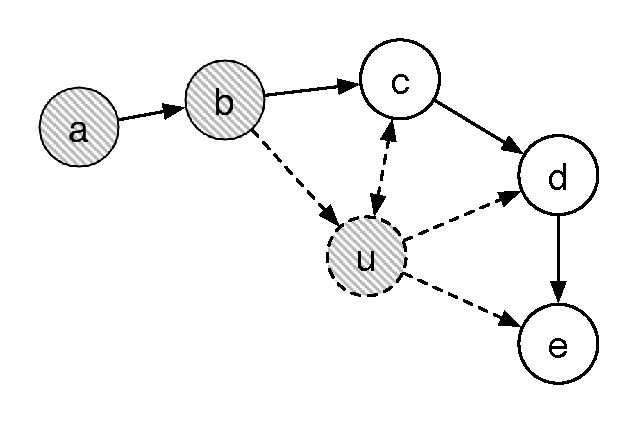
\includegraphics[width=1.0\textwidth]{figures/dyna_rm.eps}
    \caption{The diagram of ``prototypical PHI query''} 
    \label{fig:PHI}
  \end{center}
\end{figure}
	% \renewcommand\thetable{\arabic{chapter}-\arabic{table}}
% \renewcommand\thefigure{\arabic{chapter}-\arabic{figure}} 

\chapter{研究方法}
\label{cha:method} 

\section{test3}
\label{sec:test3}
	% \renewcommand\thetable{\arabic{chapter}-\arabic{table}}
% \renewcommand\thefigure{\arabic{chapter}-\arabic{figure}} 

\chapter{實驗結果與分析}
\label{cha:result} 

\section{test4}
\label{sec:test4}
	% \renewcommand\thetable{\arabic{chapter}-\arabic{table}}
%\renewcommand\thefigure{\arabic{chapter}-\arabic{figure}} 
\chapter{實驗設計}
\label{cha:dis} 

\section{test5}
\label{sec:test5}
	% \renewcommand\thetable{\arabic{chapter}-\arabic{table}}
% \renewcommand\thefigure{\arabic{chapter}-\arabic{figure}} 
\chapter{結論與後續工作}
\label{cha:work} 

\section{test6}
\label{sec:test6}


本論文蒐集了各類資訊安全工具軟體,目的是為了讓更多使用者了解資訊安全的重要性,以及如何更有效的運用網路資源。透過一系列的資訊安全基礎知識及專有名詞解釋,搭配軟體的安裝及實作步驟,讓初級使用者能更容易跨越資訊安全議題的門檻,對駭客攻防與妨駭相關知識有更深的了解(\cite{Guo2021})。

對進階使用者而言,本手冊也針對開放源碼工具做介紹,大部分工具都有釋出其原始碼,並歡迎有能力的使用者開發出更完善的程式。另外,使用者也可以結合不同功能性的軟體,自行開發出一套符合其需求的軟體,例如利用作業系統辨識工具搭配弱點掃描工具,能夠更快的找出目標主機的系統漏洞,以發揮1+1大於2的功效(\cite{test1})。

\section{Future Work} 
\label{sec:work1}

	%---------------------------------------------------------------------------------------------------------
	% back pages 後頁
	% 包括參考文獻、附錄、自傳
	% 實際內容由
	%    my_bib.bib, my_appendix.tex, my_vita.tex
	% 決定
	% ntust_backpages.tex 此檔只提供整體架構的定義,不需更動
	% 在撰寫各章草稿時,可以把此部份「關掉」,以節省無謂的編譯時間。
        
	%
% this file is encoded in utf-8
% v1


%%% 參考文獻
%%%%%%%%%%%%%%%%%%%%%%%%%%%%%%%
% 中文文獻 bib add keywords = {chinese}
%%%%%%%%%%%%%%%%%%%%%%%%%%%%%%%
\chapter*{\nameRef}
\addcontentsline{toc}{chapter}{\nameRef}
%
\phantomsection %隱藏標記 (因為\section* 不會自動增加節的編號)
\section*{中文部分}
\addcontentsline{toc}{section}{中文部分}
\printbibliography[heading=none, keyword=chinese]
%%%%%%%%%%%%%%%%%%%%%%%%%%%%%%%

%%%%%%%%%%%%%%%%%%%%%%%%%%%%%%%
% 英文文獻 bib add keywords = {english}
%%%%%%%%%%%%%%%%%%%%%%%%%%%%%%%
\newpage
\phantomsection %隱藏標記 (因為\section* 不會自動增加節的編號)
\section*{英文部分}
\addcontentsline{toc}{section}{英文部分}
\printbibliography[heading=none, keyword=english]

% \printbibliography

%%%%%%%%%%%%%%%%%%%%%%%%%%%%%%%

%%% 附錄
%%
% this file is encoded in utf-8
% v1

%%% 每一個附錄 (附錄一、附錄二、...) 都要複製此段附錄編排碼做為起頭
%%% 附錄編排碼 begin >>>
\newpage
\chapter*{附錄一:MATLAB 程式列表} % 修改附錄編號與你的附錄名
\addcontentsline{toc}{chapter}{附錄一:MATLAB 程式列表} %建議此內容應與上行相同
\renewcommand{\thechapter}{一} % 如果是附錄二,則內容應為{二}

\setcounter{equation}{0} 
\setcounter{figure}{0} 
\setcounter{footnote}{0} 
\setcounter{section}{0} 
\setcounter{subsection}{0}
\setcounter{subsubsection}{0}
\setcounter{table}{0} 
%%% <<< 附錄編排碼 end

% 附錄內容開始
\lstinputlisting{example/example_prog_list.m}


%%% 如果有附錄二、三、...,則在此繼續加上「附錄編排」碼
% 每一個附錄會自動以新頁開始

%%% 自傳
%\newpage
%\chapter*{\protect\makebox[5cm][s]{\nameVita}} % \makebox{} is fragile; need protect
%\addcontentsline{toc}{chapter}{\nameVita}
%您的自傳



%%%%%%%%%%%%%%%%%%%%%%%%%%%%%%%
%       授權書 (計頁碼,但不印頁碼) 
%%%%%%%%%%%%%%%%%%%%%%%%%%%%%%%
%
% insert the printed standard form when the thesis is ready to bind
% 在口試完成後,再將已簽名的授權書放入以便裝訂
% create an entry in table of contents for 授權書
% 目前送出空白頁
% \newpage{\thispagestyle{empty}\addcontentsline{toc}{chapter}{\nameCopyrightForm}\mbox{}\clearpage}



\end{document} 
 
